% !TEX program = xelatex
% Example: TikZ state machine (automata)
\documentclass[11pt, a4paper]{article}
\usepackage{tikz}
\usetikzlibrary{automata, positioning, arrows.meta}

\begin{document}

\section*{آلةُ حالاتٍ منتهية}

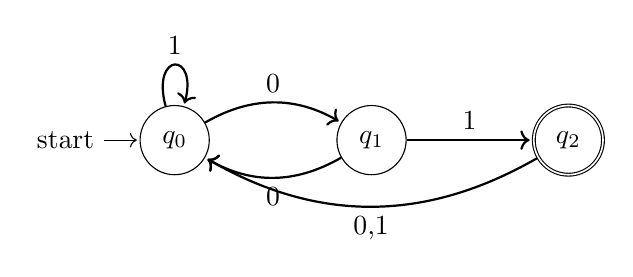
\begin{tikzpicture}[shorten >=1pt, node distance=2.5cm, on grid, auto]
  \node[state, initial] (q0) {$q_0$};
  \node[state] (q1) [right=of q0] {$q_1$};
  \node[state, accepting] (q2) [right=of q1] {$q_2$};

  \path[->, thick]
    (q0) edge [bend left] node {0} (q1)
          edge [loop above] node {1} (q0)
    (q1) edge [bend left] node {0} (q0)
          edge node {1} (q2)
    (q2) edge [bend left] node {0,1} (q0);
\end{tikzpicture}

\end{document}
